% !TeX spellcheck = en_US
\chapter{Evaluation}\label{ch:evaluation}

This chapter presents the evaluation of the several approaches presented in Ch.~\ref{ch:approach} and~\ref{ch:implementation}.  First, the performances of GRP and HDT are compared. Second, the proposed compression improvements are evaluated.

For the following experiments, HDT-Java 2.0~\footnote{\label{foot:1}https://github.com/rdfhdt/hdt-java/releases/tag/v2.0} (the currently newest version) has been used. For GRP the implementation presented in Ch.~\ref{sec:relatedworkGRPImpl} has been used. The evaluated datasets are the ones introduced in Ch.~\ref{sec:implementationDatasets}.


\section{GRP vs HDT}\label{sec:evaluationHDTvsGRP}

This chapter shows the evaluation results of the comparison between HDT and GRP. First, results for the synthetically generated graphs from Ch.~\ref{sec:implementationGRPvsHDT} will be presented. Afterwards, the two compressors will also be evaluated for real world data.

\begin{figure}[h]
	\centering
	\subfloat[$CR_{Graph_{HDT}}$ and $CR_{Graph_{GRP}}$.]{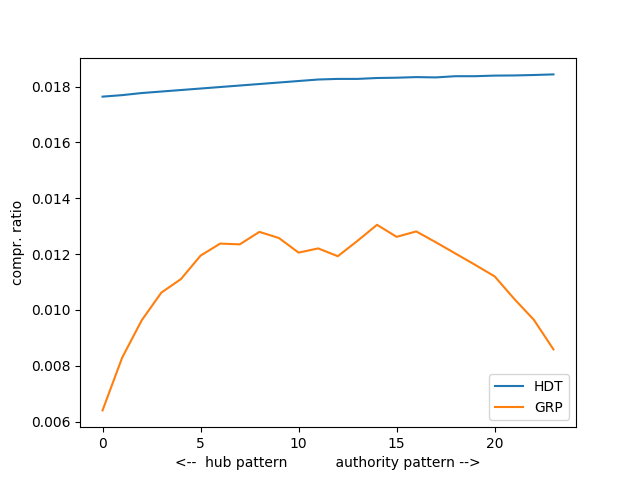
\includegraphics[width=\subfigCurvePlotWidth\textwidth]{figures/GRPvsHDT/bothWithoutDict}\label{fig:ratiosBothWithoutDict}}
	\hfill 
	\subfloat[$CR_{HDT}$ and $CR_{GRP}$.]{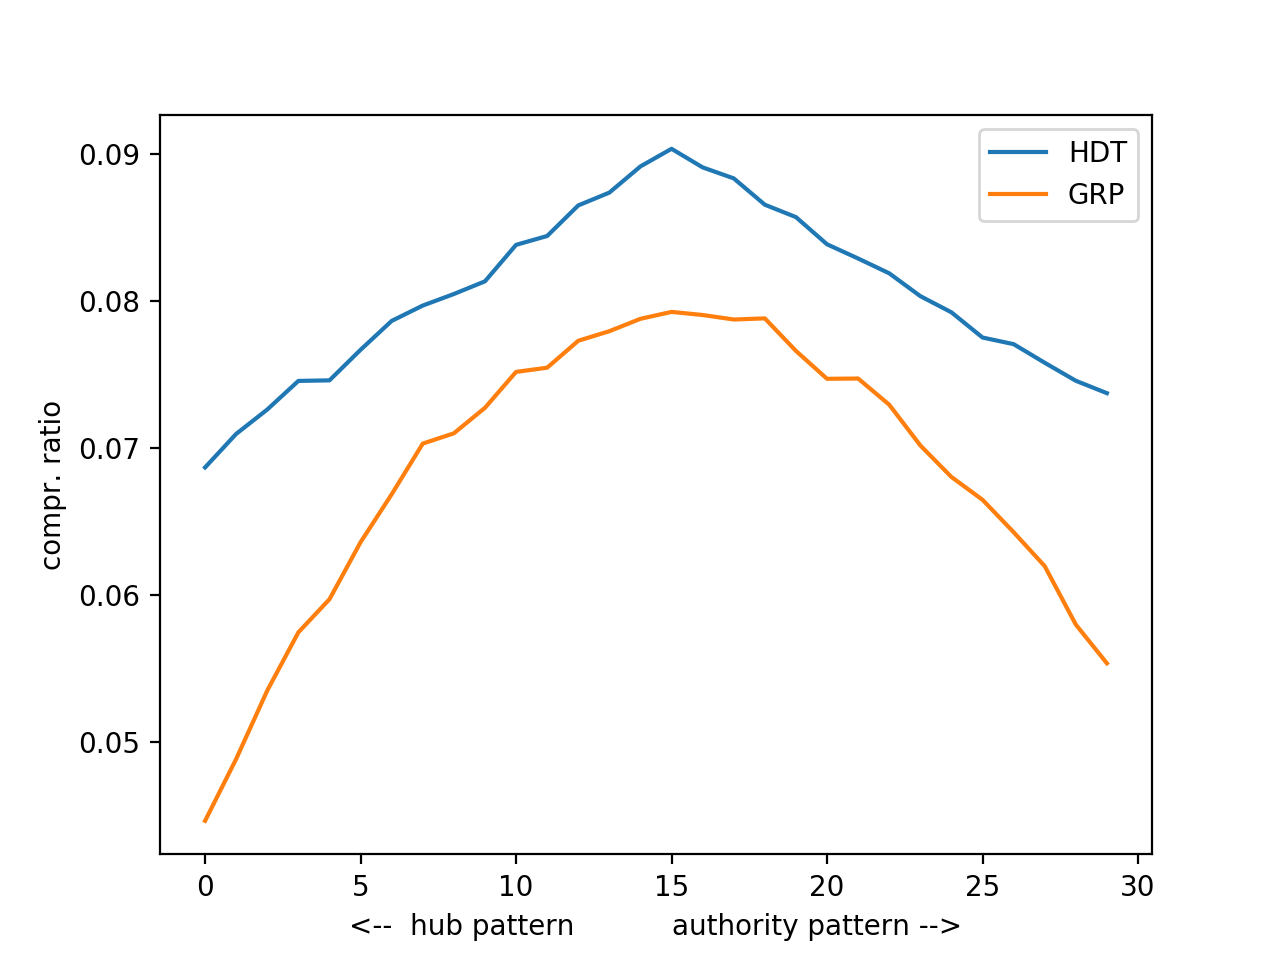
\includegraphics[width=\subfigCurvePlotWidth\textwidth]{figures/GRPvsHDT/bothWithDict}\label{fig:ratiosBothWithDict}}
	\caption{The compression ratios for GRP and HDT without and with dictionary sizes.}
	\label{fig:grpvshdt1}
\end{figure}

\subsection{Results for Synthetic Data}

Fig.~\ref{fig:grpvshdt1} shows the results for the synthetically generated data (see Ch.~\ref{sec:implementationGRPvsHDT}). Fig.~\ref{fig:ratiosBothWithoutDict} shows \CRGraph{C} (without the size of the dictionary). As expected, $CR_{Graph_{HDT}}$ becomes higher, as the graphs are further away from the hub pattern. Moreover, \GGRP{} compresses better if the graph is similar to the star pattern (greater value of $SPS$), as stated earlier. It is noticeable that $CR_{Graph_{GRP}}$ fluctuates much more than $CR_{Graph_{HDT}}$ and the impact of the star pattern similarity is much higher for \GGRP{}.


Fig.~\ref{fig:ratiosBothWithDict} shows the values of \CR{HDT} and \CR{GRP}. It can be seen that the curves behave differently than in Fig.~\ref{fig:ratiosBothWithoutDict}, since the dictionary size $|out_{dict}|$ is much bigger than $|out_{graph}|$. As both GRP and HDT use the same dictionary compressor ($Dict_{HDT}$), they have been increased by the same amount and therefore \CR{GRP} is smaller than \CR{HDT}. Furthermore, it is noticeable that $|out_{dict}|$ is bigger when the graph is further away from the star pattern. This is due to the fact that the number of different URIs becomes higher at a lower value of $SPS$, because of the way these graphs are constructed (see Fig.~\ref{fig:rdfFile}).

\begin{figure}
	\centering
	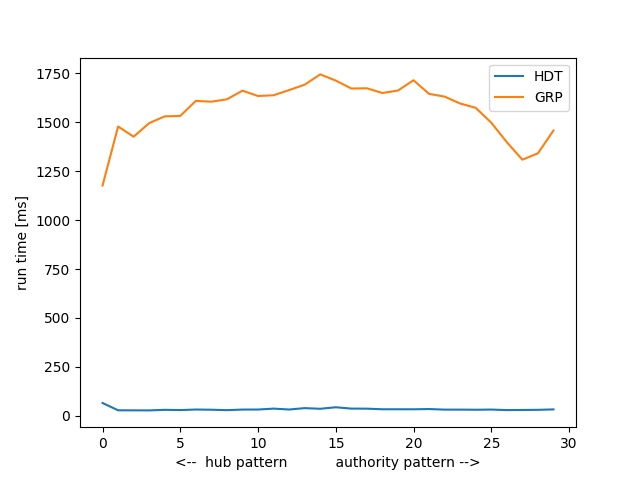
\includegraphics[width=0.7\linewidth]{figures/GRPvsHDT/runtimes}
	\caption{$CT_{HDT}$ and $CT_{GRP}$ (Average run time of 100 consecutive executions).}
	\label{fig:runtimes}
\end{figure}

Apart from the compression ratio, the run time is also important for the overall performance. Fig.~\ref{fig:runtimes} shows the average value of $CT$ for both compressors, respectively. Here, the same scenario with the star pattern (and only one distinct predicate) was used. It has been executed 100 times to get a sophisticated run time measurement, because $CT$ depends on the current CPU workload of the computer. Decompression is not supported by the currently implemented version of GRP and will therefore be omitted. It can be seen that $CT_{GRP}$ is on average 48 times higher than $CT_{HDT}$. However, it should also be noted that the implementation of GRP is rather rudimentary  (according to the authors of~\cite{maneth}), while that of HDT has been under development for some time. So, they are not on the same level in terms of quality. In theory, GRP should be able to compete with HDT, since it has linear run time with respect to the size of the graph~\cite{maneth}. In~\cite{hdt}, the authors do not mention HDT's run time in $\mathcal{O}$-notation.
\FloatBarrier

In Ch.~\ref{sec:implementationGRPvsHDT}, it was mentioned that only one distinct predicate will be used in the first comparison. However, in the following it is shown how the compressors behave as the number of predicates increases. To realize that, the whole procedure from Ch.~\ref{sec:implementationGRPvsHDT} is executed  four times with an increasing number of predicates each time. The plots for those executions are shown in Fig.~\ref{fig:bothwithoutdictincreasingpreds}. For both algorithms, the $CR_{Graph_C}$-values get bigger as the number of predicates increases. The curves with same line styles have to be compared, since those pairs have the same number of predicates. The fourth execution is marked by the solid red lines and this is the first case in which $CR_{Graph_{HDT}} <CR_{Graph_{GRP}} $ is true. So, there are cases in which \GHDT{} compresses better. That continues, as the number of predicates is further increased. Hence, higher amounts of predicates have a higher impact on \GGRP{} than on \GHDT{}. However, the next chapter will show that there is no fixed value for $ELR$ at which \GHDT{} is always better.

\begin{table}[ht]
	\begin{minipage}[b]{1\linewidth}
		\centering
		\begin{tabular}{|c|c|}
			\hline 
			Iteration & Line Style \\ 
			\hline 
			1 & $ \cdot \cdot$ \\ 
			\hline 
			2 & -- -- \\ 
			\hline 
			3 & \rotatebox[origin=c]{-180}{$\triangle \triangle$} \\ 
			\hline 
			4 & --- \\ 
			\hline 
		\end{tabular}
		\caption{Legend for the line styles in Fig.~\ref{fig:bothwithoutdictincreasingpreds}. A higher iteration number indicates a higher number of predicates.}
		\label{tab:legend}
	\end{minipage}\hfill
	\begin{minipage}[b]{\linewidth}
		\centering
		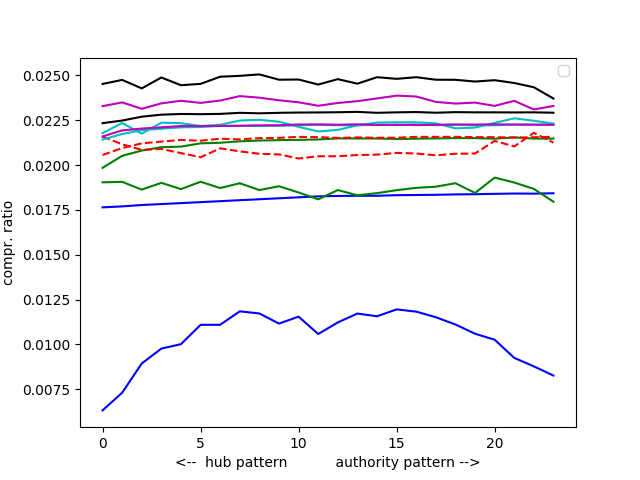
\includegraphics[width=\linewidth]{figures/GRPvsHDT/bothWithoutDictIncreasingPreds}
		\captionof{figure}{$CR_{Graph_C}$-values for HDT and GRP. Same line styles indicate that the number of distinct predicates is the same (legend is shown in Tab.~\ref{tab:legend}). The two solid lines (iteration 4) show the first case in which $CR_{Graph_{HDT}} <CR_{Graph_{GRP}} $ holds.}
		\label{fig:bothwithoutdictincreasingpreds}
	\end{minipage}
\end{table}

\FloatBarrier
\subsection{Results for Real World Data}

The previous chapter used synthetic data to detect the behavior of the compressors to certain changes in the structure of the input data. Next, real data will be used to compare the compression ratios of \GHDT{} and \GGRP{}. 

\subsubsection{Dataset Overview}

Here, an overview of the used RDF files is provided. They are contained in the following datasets: DBPedia, Semantic Web Dog Food, WikiData and Open Government Data. Tab.~\ref{tab:comparisonDatasets} shows the files that are used, as well as their number of triples and resources. Also, their values for $ELR$ and $SPS$ are shown. It has to be noted that the entity-based sub graphs are limited to 50000 triples.

\FloatBarrier
\begin{center}
	\begin{tabular}{|c|c|c|c|c|c|}
		\hline 
		Short Name & Long Name & \#Triples & \#Resources & $ELR$ & $SPS$ \\ 
		\hline
		DF0 & dc-2010-complete-alignments & 5919 & 821 & 0.008 & 0.000043 \\
		\hline
		DF1 & ekaw-2012-compl-alignments & 13114 & 1604 & 0.004 & 0.052 \\
		\hline
		DF2 & eswc-2006-compl-alignments & 6654 & 1259 & 0.004 & 0.071 \\
		\hline
		DF3 & eswc-2009-compl-alignments & 9462 & 1247 & 0.004 & 0.054 \\
		\hline
		DF4 & eswc-2010-compl-alignments & 18122 & 2226 & 0.002 & 0.091 \\
		\hline
		DF5 & eswc-2011-compl-alignments & 25865 & 3071 & 0.002 & 0.114 \\
		\hline
		DF6 & iswc-2002-compl-alignments & 13450 & 1953 & 0.003 & 0.057 \\
		\hline
		DF7 & iswc-2003-compl-alignments & 18039 & 2565 & 0.002 & 0.102 \\
		\hline
		DF8 & iswc-2005-compl-alignments & 28149 & 3877 & 0.001 & 0.132 \\
		\hline
		DF9 & iswc-2010-compl-alignments & 32022 & 3842 & 0.001 & 0.116 \\
		\hline 
		\hline
		DB0 & external-links\_en & 50000 & 54931 & 2.0E-5 & 0.038 \\
		\hline
		DB1 & geo-coordinates\_en & 50000 & 12505 & 8.0E-5 & 0.2 \\
		\hline
		DB2 & homepages\_en & 50000 & 98584 & 2.0E-5 & 0.006 \\
		\hline
		DB3 & instance-types-transitive\_en & 50000 & 7722 & 2.0E-5 & 0.229 \\
		\hline
		DB4 & instance-types\_en & 50000 & 35677 & 2.0E-5 & 0.387 \\
		\hline
		DB5 & mappingbased-properties\_en & 50000 & 21590 & 0.01502 & 0.028 \\
		\hline
		DB6 & persondata\_en & 50000 & 10631 & 1.8E-4 & 0.112 \\
		\hline
		DB7 & transitive-redirects\_en & 50000 & 82318 & 2.0E-5 & 0.022 \\
		\hline
		\hline
		OD0 & 00f1dbeb-4ba1-4dac-92ec & 50000 & 6094 & 4.39E-4 & 0.294 \\
		\hline
		OD1 & 4eb92c99-76fe-4987-a475 & 50000 & 6613 & 1.99E-4 & 0.23 \\
		\hline
		OD2 & 95414599-bfc3-4472-931f & 50000 & 5349 & 3.59E-4 & 0.376 \\
		\hline
		OD3 & ac7e4a31-ab86-496b-98a9 & 50000 & 5349 & 3.59E-4 & 0.376 \\
		\hline
		OD4 & e4342f74-dd87-4667-8c31 & 50000 & 6616 & 1.99E-4 & 0.247 \\
		\hline
		\hline
		WD0 & wikidata-20190426-lexemes & 50000 & 9443 & 0.004 & 0.201 \\
		\hline
		WD1 & wikidata-20190510-lexemes & 50000 & 9569 & 0.004 & 0.2 \\
		\hline
		WD2 & wikidata-20190517-lexemes & 50000 & 9729 & 0.004 & 0.2 \\
		\hline
		WD3 & wikidata-20190524-lexemes & 50000 & 9740 & 0.004 & 0.2 \\
		\hline
		WD4 & wikidata-20190607-lexemes & 50000 & 9742 & 0.004 & 0.2 \\
		\hline
	\end{tabular} 
	\captionof{table}{RDF files for the comparison of GRP and HDT. URLs to the datasets are in Ch.~\ref{sec:implementationDatasets}.}	
	\label{tab:comparisonDatasets}
\end{center}

\FloatBarrier

On most of the used RDF graphs, \GGRP{} achieves a better compression ratio than \GHDT{}. On average, $CR_{Graph_{HDT}}$ is 1.8 times higher than $CR_{Graph_{GRP}}$.

In order to investigate the correlation between the pairs ($CR_{Graph_C},ELR$) and ($CR_{Graph_C},SPS$) the Spearman correlation is used. That correlation coefficient produces values between $ -1 $ and $ 1 $. Negative values imply a negative correlation, positive values imply a positive correlation. The value 0 means that there is no correlation.~\cite{spearman} 

The results are shown in Tab.~\ref{tab:spearman}. Due to the value $0.646$ it becomes clear that higher numbers of different predicates lead to a higher compression ratio for $Graph_{GRP}$. In contrast, a higher value of $SPS$ implies a lower compression ratio for $Graph_{GRP}$, as expected. Although it has to be noted that for the latter case, the correlation is not as strong as with $ELR$. 

$CR_{Graph_{HDT}}$ has a positive correlation with $ELR$, but that correlation is quite small. The correlation between $CR_{Graph_{HDT}}$ and $SPS$ is positive (but very close  to 0) which is reasonable, since $Graph_{HDT}$ only benefits from hub pattern, but $SPS$ is defined for the general star pattern.

\begin{figure}[h]
	\centering
	\subfloat[DBPedia]{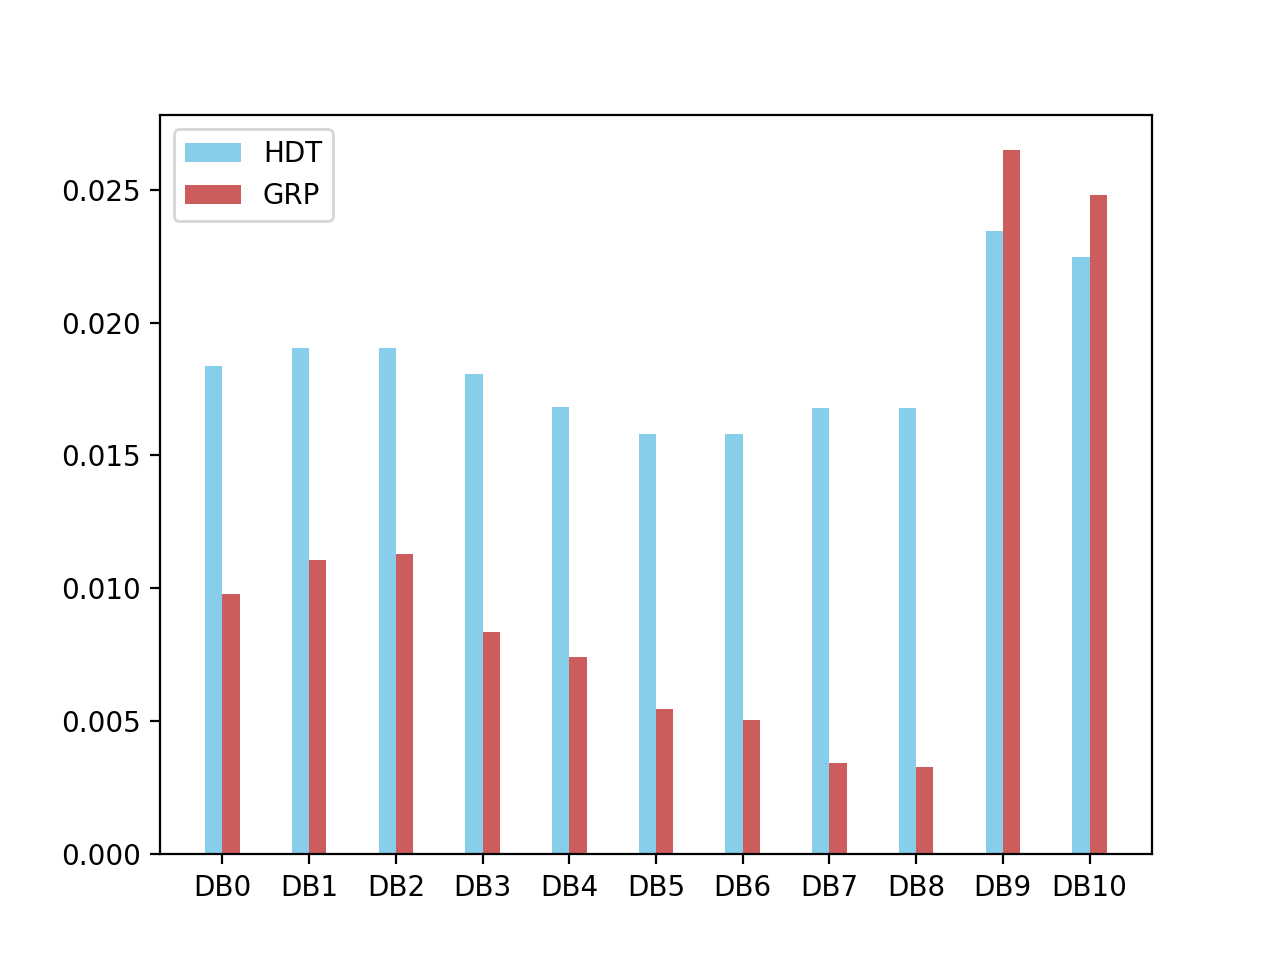
\includegraphics[width=\subfigWidth\textwidth]{figures/GRPvsHDT/realdata/dbpedia}\label{fig:compare1a}}
	\hfill
	\subfloat[Semantic Web Dog Food]{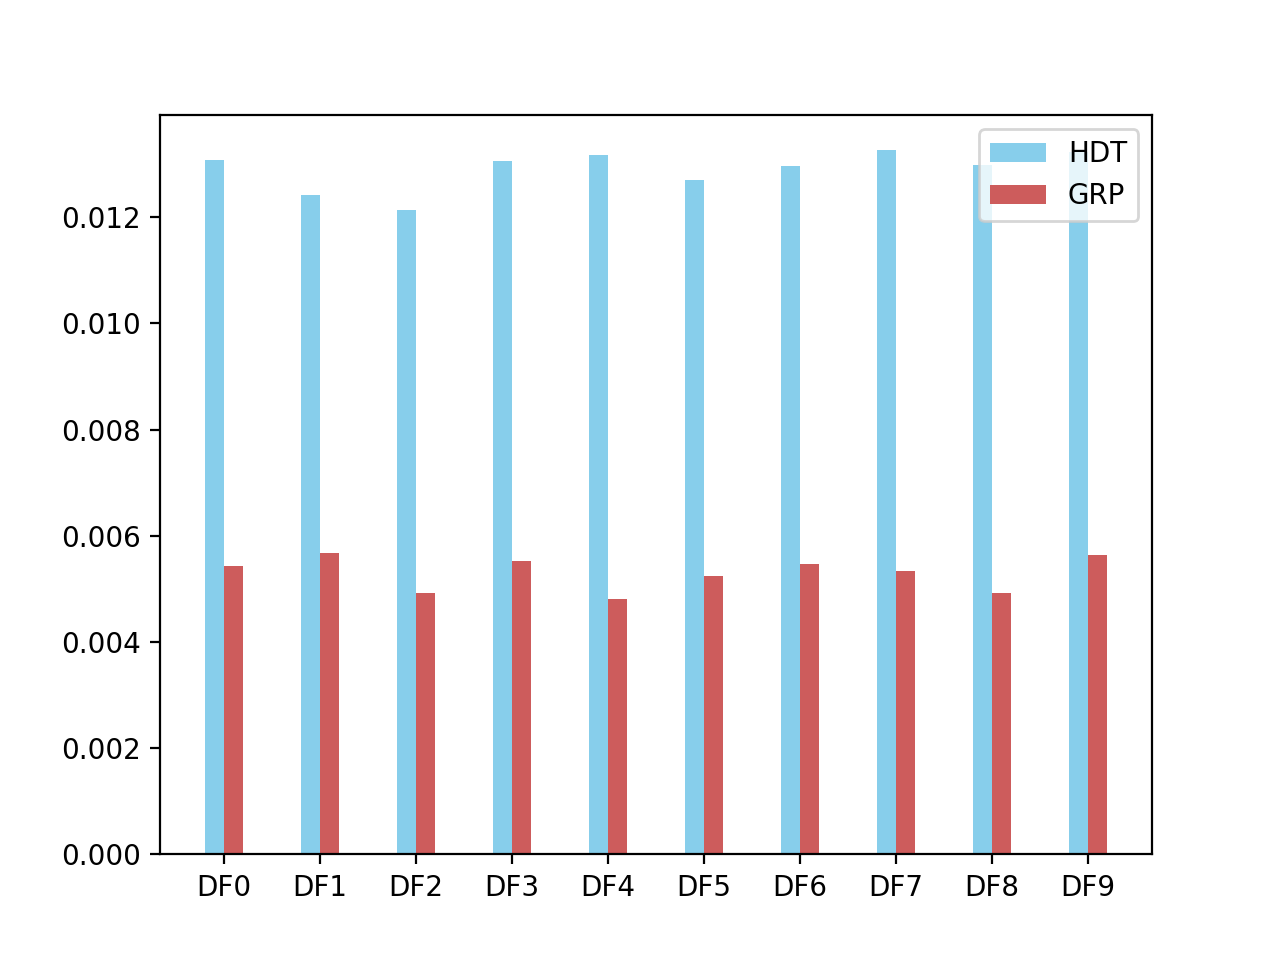
\includegraphics[width=\subfigWidth\textwidth]{figures/GRPvsHDT/realdata/dogfood}\label{fig:figcompare1b}}
	\caption{$CR_{Graph{HDT}}$ and $CR_{Graph{GRP}}$.}
	\label{fig:compare1}
\end{figure}

\todo{werte mit vorsicht genießen}
\begin{center}
	\begin{tabular}{|c|c|c|}
		\hline 
		& $CR_{Graph_{GRP}}$ & $CR_{Graph_{HDT}}$ \\ 
		\hline 
		$ELR$ & $ 0.646 $ & $ 0.181 $  \\ 
		\hline 
		$SPS$ & $ -0.381 $ & $ 0.009 $ \\ 
		\hline 
	\end{tabular} 
	\captionof{table}{Spearman correlation values.}	
	\label{tab:spearman}
\end{center}

Fig.~\ref{fig:compare1} and~\ref{fig:compare2} show the compression ratios for the datasets, respectively. It has to be noticed that values of $CR_{Graph_C}$ are not comparable between different RDF files. This is due to the fact that $CR_{Graph_C}$ does not take the dictionary into account. Hence, if two files $f_1,f_2$ have the same graph structure, but $f_1$  is using longer URIs than $f2$, then $CR_{Graph_C}$ will be smaller for $f_1$. This is because $|f_1|>|f_2|$ is true and $CR_{Graph_C}=\frac{out_{graph}}{in}$ (with $in\in \{f_1,f_2\}$ in this case). Therefore, the compression ratios of the two approaches can only be compared if they were achieved on the same input file.


\begin{figure}[h]
	\centering
	\subfloat[Government Open Data]{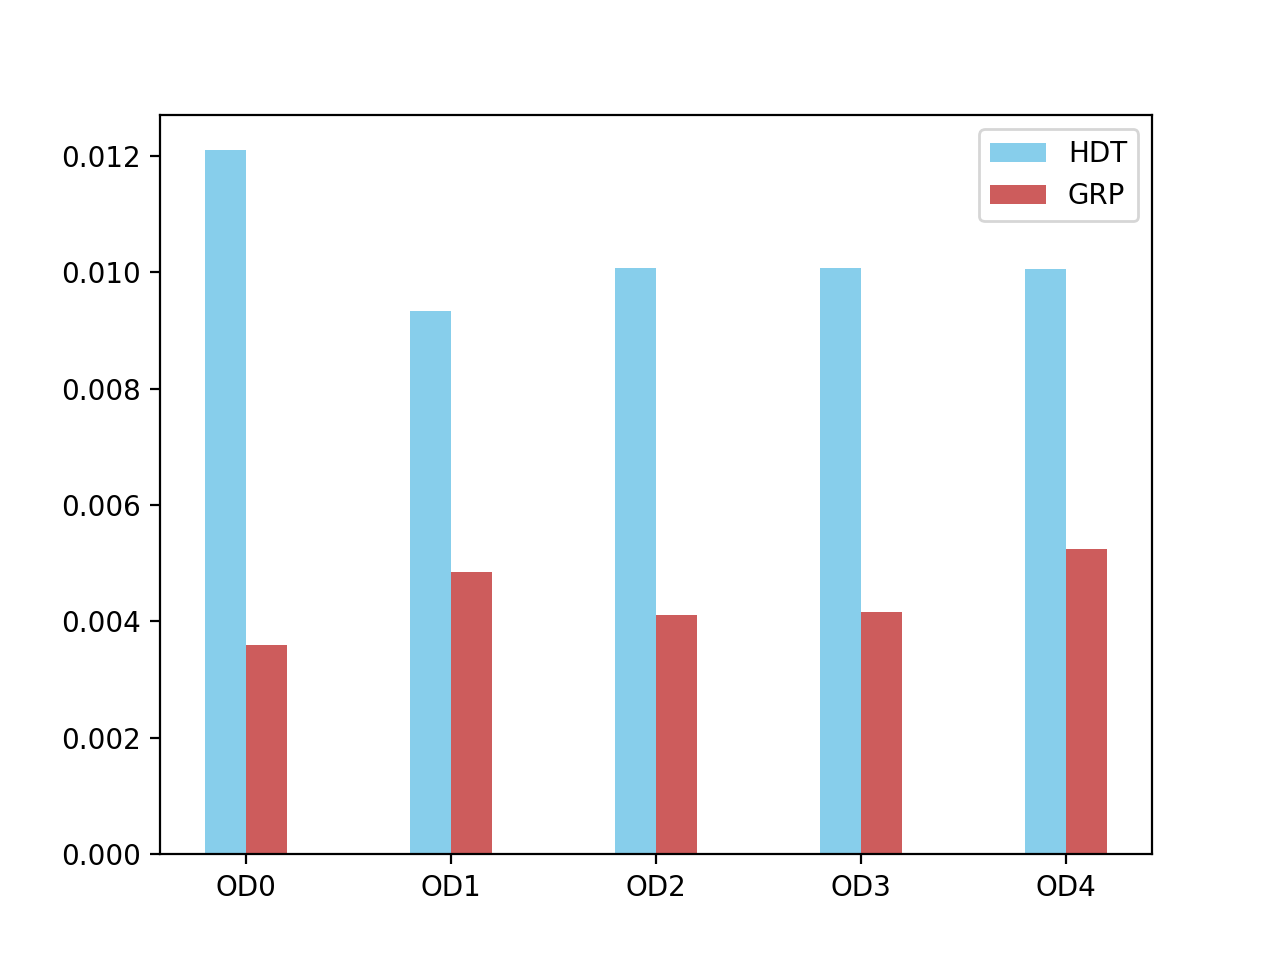
\includegraphics[width=\subfigWidth\textwidth]{figures/GRPvsHDT/realdata/opendata}\label{fig:compare2a}}
	\hfill
	\subfloat[WikiData]{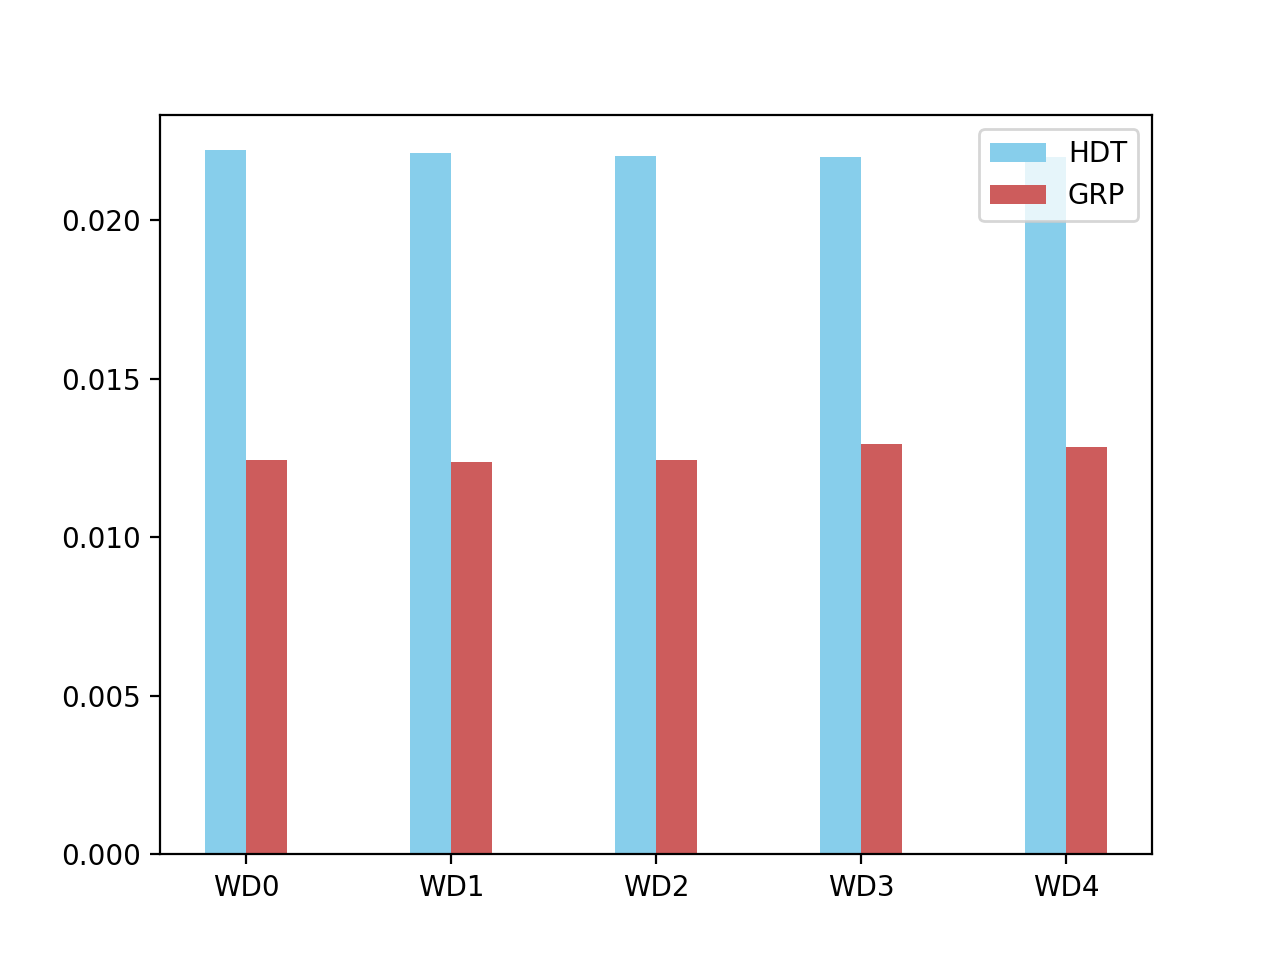
\includegraphics[width=\subfigWidth\textwidth]{figures/GRPvsHDT/realdata/wikidata}\label{fig:figcompare2b}}
	\caption{$CR_{Graph{HDT}}$ and $CR_{Graph{GRP}}$.}
	\label{fig:compare2}
\end{figure}

\section{Compression Improvements}

This chapter shows the evaluation results for the compression improvements. First, results for the graph compression improvements (\GGRP)  are discussed. Then, results for the dictionary compression improvements (\DHDT) are presented.  In the end, both approaches will be combined in a final evaluation.

\subsection{Ontology Knowledge}\label{sec:evaluationOntKnowledge}

In this chapter, it will be evaluated whether using meta data from the ontology can result in a better compression ratio for $Graph_{GRP}$. Here, not only the file size of the output ($|out_{graph}|$) will be measured. Since these approaches have the intention to improve the ability for $Graph_{GRP}$ to produce a smaller grammar, the features of that grammar will be presented in more detail. That is because the GRP's grammar encoding does not always produce a smaller result on a smaller graph (as mentioned in Ch.~\ref{sec:related_workGrammarEncoding}).

\subsubsection{Dataset Overview}

Tab.~\ref{tab:ontologyKnowledgeDatasets} shows an overview of the data used for the ontology-based manipulations. \textit{MBP} stands for \textit{mappingbased-properties\_en}. $DB_{full}$ is the full version of \textit{MBP} and $WN_{full}$ is the full version of Wordnet. The other datasets are adjusted to show the effects of the manipulations better. They contain a higher proportion of symmetric, inverse or transitive properties, respectively.

\begin{center}
	\begin{tabular}{|c|c|c|c|c|c|}
		\hline 
		Short Name & Long Name & \#Triples & \#Resources & $ELR$ & $SPS$ \\ 
	    \hline
		$DB_{full}$ & MBP& 32018293 & 4803076 & 0.04 & 0.158 \\
		\hline
	    $DB_{inv}$ & MBP\_manyinverses & 1097 & 935 & 0.037 & 0.022 \\
		\hline
		$DB_{sym}$ & MBP\_manysymmetrics & 19954 & 18785 & 0.008 & 0.037 \\
		\hline
		$DB_{tra}$ & MBP\_manytransitives & 1994 & 1147 & 0.101 & 0.0004 \\
		\hline
		\hline
		$WN_{full}$ & wordnet & 2637168 & 601641 & 0.0 & 0.223 \\
		\hline
		$WN_{inv}$ & wordnet\_manyinverses & 1999 & 1351 & 0.008 & 0.113 \\
		\hline
		$WN_{sym}$ & wordnet\_manysymmetrics & 1999 & 2283 & 0.003 & 0.058 \\
		\hline
		$WN_{tra}$ & wordnet\_manytransitives & 3988 & 2033 & 0.004 & 0.08 \\
		\hline
	\end{tabular} 
	\captionof{table}{RDF files for the ontology-based improvements. URLs to the datasets are in Ch.~\ref{sec:implementationDatasets}.}	
	\label{tab:ontologyKnowledgeDatasets}
\end{center}

\subsubsection{Occurrence of Properties}

In the following, symmetric, inverse or transitive properties are called relevant properties.

First, it is considered which relevant properties occur in real world datasets. Tab.~\ref{tab:ontologyKnowledgeRelevantProperties} shows the relevant properties for DBPedia and Wordnet. It can be concluded that these amounts are relatively small, especially for symmetric properties, considering the fact that these datasets are relatively large. 

Next, it is considered how often the relevant properties occur in the datasets.  Thus, $DB_{full}$ and $WN_{full}$ will be analyzed. Fig.~\ref{fig:ontoccurrences} shows how often the relevant properties occur. (Relative amount = $\frac{\text{\#occurrences}}{\text{\#triples}}$). It can be noticed that the amounts are quite low. This supports the hypothesis from Ch.~\ref{sec:implementationOntKnowledge} that building sub graphs with higher amounts of relevant properties is necessary to observe the effect of the data manipulations. Consequently, those sub graphs (see Ch.~\ref{sec:implementationSubGraphs}) are used in the following evaluations.

\begin{center}
	\begin{tabular}{|c|c|c|}
		\hline 
		& DBPedia & Wordnet \\ 
		\hline 
		URL Prefix & \makecell{http://dbpedia.org/\\ontology/} & \makecell{http://wordnet-rdf.princeton.edu/\\ontology\#} \\
		\hline
		Symmetric & spouse & antonym \\ 
		\hline 
		Inverse & \makecell{(doctoralStudent, doctoralAdvisor)\\(mother, child)\\(father, child) \\(follows, followedBy)} & (hypernym, hyponym) \\ 
		\hline 
		Transitive & \makecell{isPartOf\\province\\locatedInArea\\city\\district\\county\\settlement} & \makecell{cause\\substance\_holonym\\part\_holonym\\entail\\member\_holonym\\member\_meronym\\instance\_hypernym\\instance\_hyponym\\hyponym\\par\_meronym\\substance\_meronym\\hypernym} \\ 
		\hline 
	\end{tabular} 
	\captionof{table}{Overview of the relevant properties of DBPedia and Wordnet.}	
	\label{tab:ontologyKnowledgeRelevantProperties}
\end{center}

\begin{figure}
	\centering
	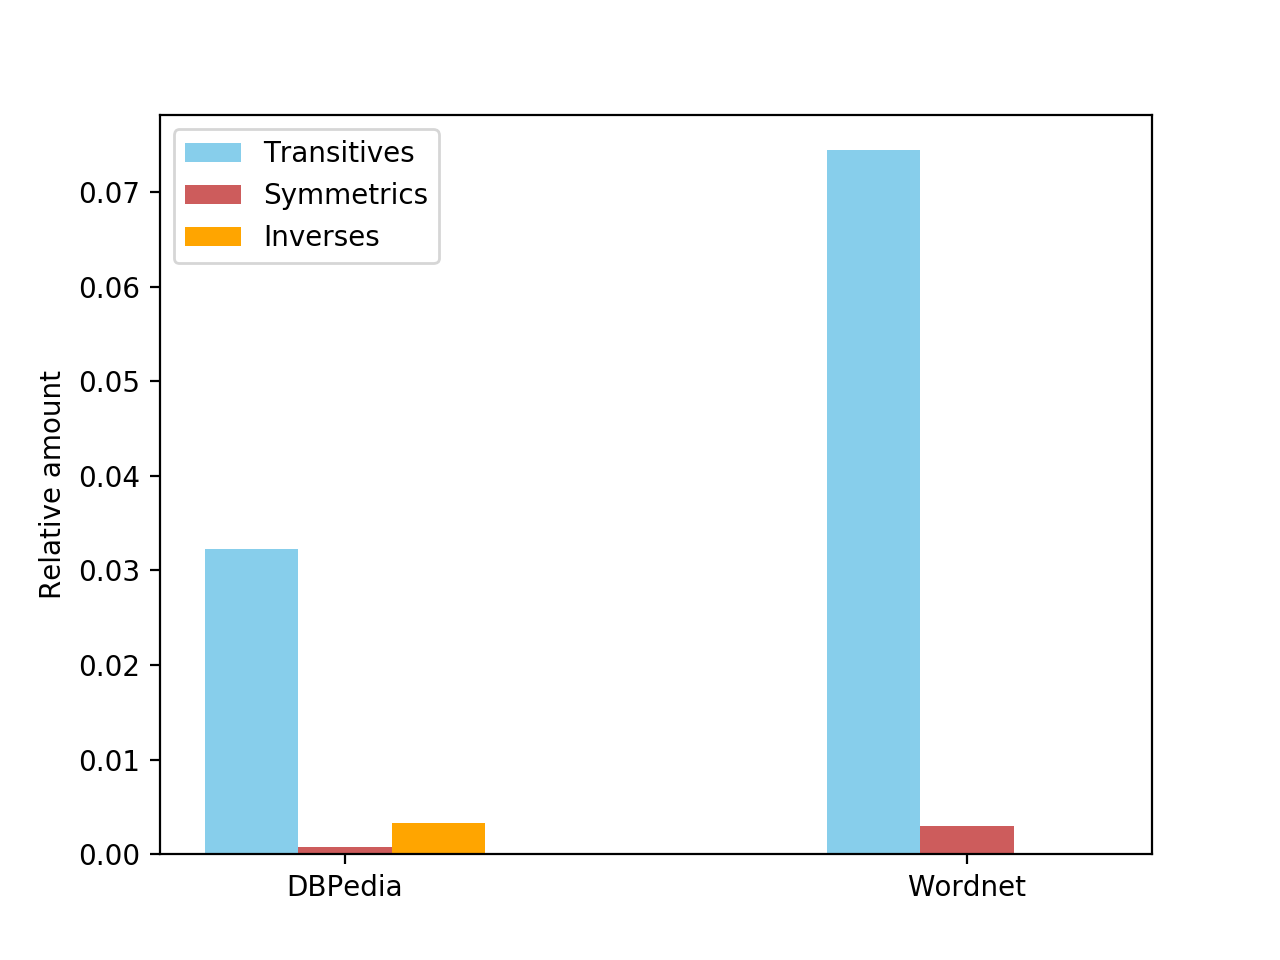
\includegraphics[width=0.7\linewidth]{figures/4_evaluation/ontOccurrences}
	\caption{Relative amount of transitive/symmetric/inverse properties in real datasets.}
	\label{fig:ontoccurrences}
\end{figure}

\pagebreak
\subsubsection{Evaluation Process}
The overall process, which is used to evaluate the ontology-based manipulations, is illustrated in Fig.~\ref{fig:overallprocess}. First, the original graph or sub graph is given to GRP. That part is called $in_1$ in Fig.~\ref{fig:overallprocess} and it will deliver the first result $out_1$.

In the next step, relevant properties have to be determined and the original graph will be manipulated. The manipulated graph is shown in the lower part of $in_2$. That manipulation step can be seen as a pre-processing and is not explicitly shown in Fig.~\ref{fig:overallprocess}. In addition, the relevant ontology triples (upper part of $in_2$) have to be compressed and stored as well. Otherwise, the original graph could not be restored. The manipulated graph and all relevant ontology triples are merged into one graph ($in_2$), which is then compressed by GRP and the result is called $out_2$. 

Finally, $out_1$ and $out_2$ have to be compared. The next chapter will explain how that is done.

\begin{figure}
	\centering
	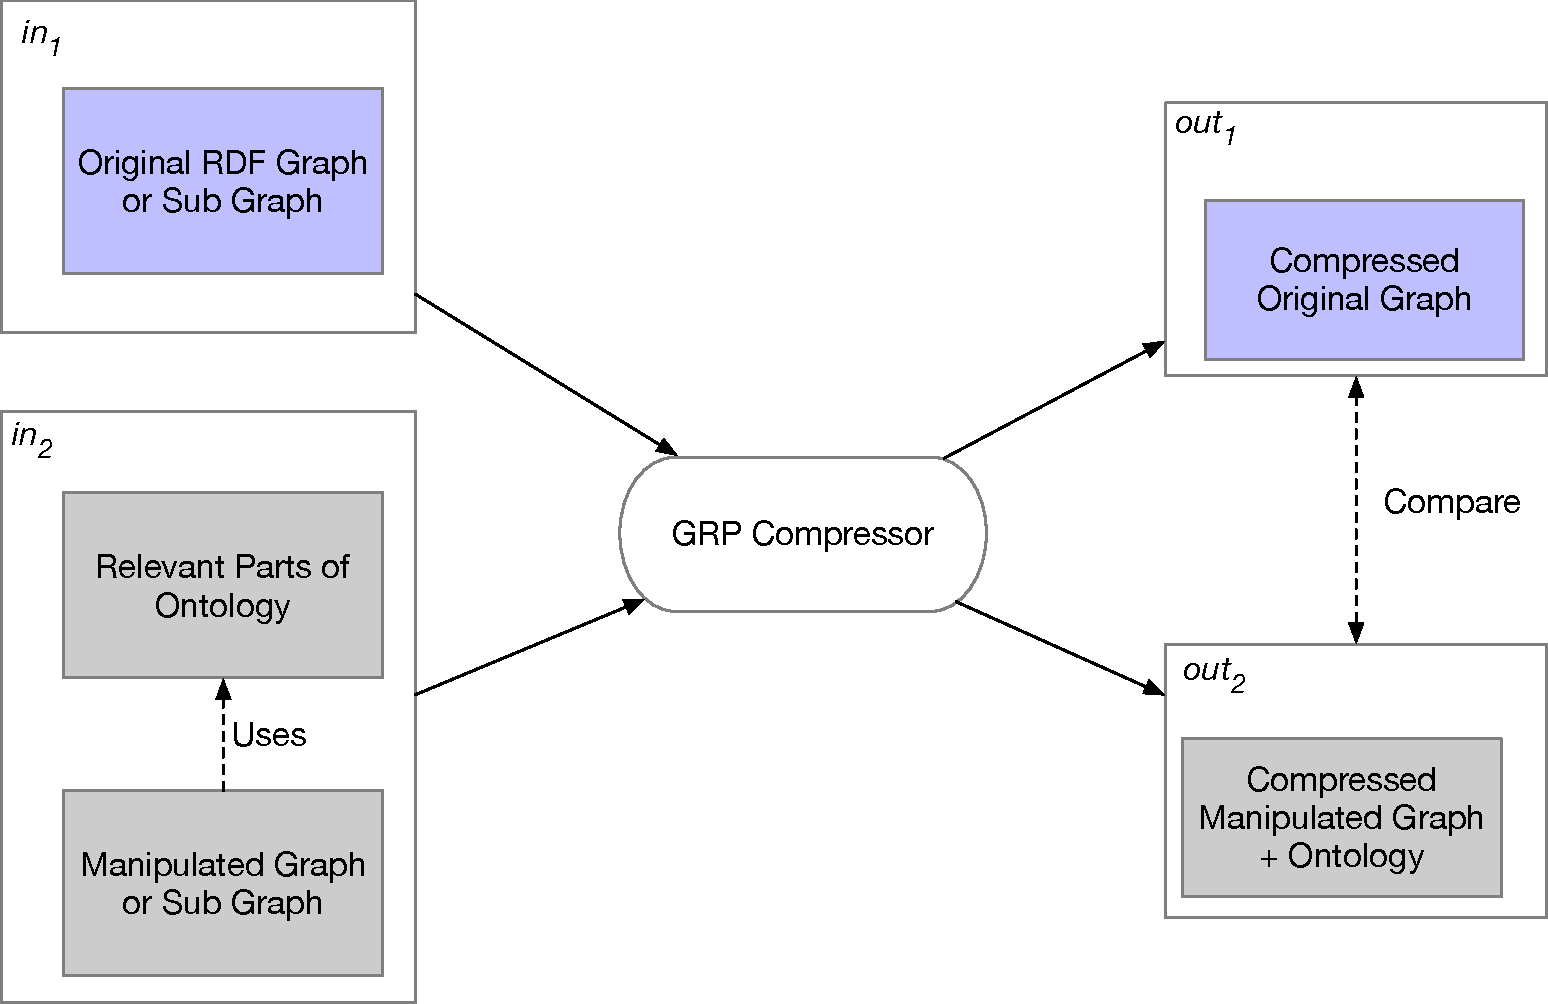
\includegraphics[width=0.8\linewidth]{figures/4_implementation/overallProcess}
	\caption{Overall process of applying ontology knowledge and comparing the compression results.}
	\label{fig:overallprocess}
\end{figure}

The evaluation process must be executed for the different manipulation aspects (symmetric, inverse etc.) independently. So, there is one manipulated graph where all symmetric edges are added or removed, and analogously for the other manipulations. This way, it is noticeable which effect the manipulations have, individually. A combined evaluation will be done in Ch.~\ref{sec:evaluationFinal}.

\subsubsection{Metrics}

This chapter explains how the two outputs $out_1$ and $out_2$ are compared. Since the ontology-based manipulations are intended to achieve a better compression ratio by enabling $Graph_{GRP}$ to produce a smaller grammar, $out_1$ and $out_2$ are not only compared at the file size level, but also in terms of their graph sizes. A reasonable metric for the size of a graph is its number of edges. In order to compare $out_1$ and $out_2$ with respect to their edge amounts, the metrics Input Edge Ratio ($IER$) and Output Edge Ratio ($OER$)  are defined: 

\begin{align*}
IER&=\frac {\text{\#edges in } in_2} {\text{\#edges in  } in_1}
\\\\
OER&=\frac {\text{\#edges in } out_2} {\text{\#edges in } out_1}
 \end{align*}
 
$IER$ shows how many edges have been added or removed by the manipulation which indicates how big the impact of the manipulation is. $OER$  shows whether the manipulation results in a better ($OER<1$) or worse ($OER>1$) compression ratio.

In order to measure the manipulation it is necessary to define a new metric instead of re-using \CRGraph{GRP} as defined in Ch.~\ref{sec:compressorModel}. For $out_1$, \CRGraph{GRP} would be in relation to $in_1$ (analogously for $out_2$ and $in_2$). But here it is necessary to compare $out_1$ and $out_2$. Therefore, the new metric Size Ratio ($SR$) is defined as follows:

\begin{align*} 
SR=\frac {|out_{graph_2}|} {|out_{graph_1}|}
\end{align*}

Here, $out_{graph}$ is used instead of $out$. Normally, the dictionary size ($out_{dict}$) should also be taken into account, because the added ontology triples have increased $|out_{dict_2}|$. However, due to the very small amount of relevant properties that increase is not even noticeable and can be omitted. 

If $SR<1$ holds then the manipulation has resulted in an improvement at the file size level, otherwise not. Of course, the file size level is, in the end, more relevant than the grammar level, because it is the size needed to store the compressed data.

\clearpage
\subsubsection{Symmetric Properties}

First, the approach suggested in Ch.~\ref{sec:approachOntKnowledge} to add all possible triples with symmetric edges will be evaluated. Fig.~\ref{fig:symmetricAddResults} illustrates the results whereby $DB_{sym}$ and $WN_{sym}$ are used for DBPedia and Wordnet, respectively. As expected, $IER$ is bigger than 1, as edges have been added to the graph. For both DBPedia and Wordnet, $IER$ is about 1.4. Also, it can be noticed that $OER<1$ holds, which means that adding symmetric triples is indeed beneficial for \GGRP{} and even brings a significant improvement on the grammar level as $OER$ is about 0.8 for DBPedia and about 0.5 for Wordnet.

Furthermore, $SR<1$ is true. Hence, also on the file size level the manipulation has delivered a better result. However, the improvement is not as good as on the grammar level. So, the statement from Ch.~\ref{sec:related_workGrammarEncoding}, that GRP's encoding method does not always work well, is supported by these results. 



\begin{figure}
	\centering
	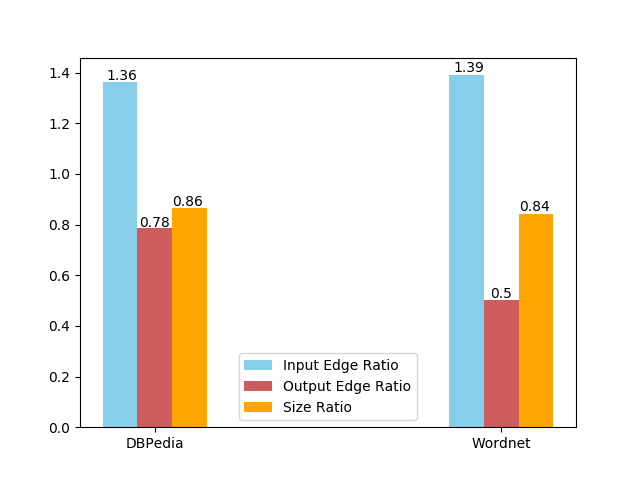
\includegraphics[width=0.8\linewidth]{figures/4_evaluation/ontology/ratiosSymmetricsAdd}
	\caption{Results for adding symmetric properties, on the grammar level ($IER$, $OER$) and on the file size level ($SR$).}
	\label{fig:symmetricAddResults}
\end{figure}


In order to show that adding symmetric properties is more beneficial than removing them, the results of the removal case are also shown (see Fig.~\ref{fig:symmetricDeleteResults}). There, it can be seen that $IER<1$ holds, since edges have been removed. But $IER$ is still quite close to 1, because there are not many cases in which an edge could be removed. Hence, in most cases only one of the two directions for symmetric properties is present in the graph. Both $OER$ and $SR$ are close or equal to 1, which indicates that adding symmetric edges is more beneficial for $Graph_{GRP}$. Nevertheless, it can still be argued that there are only a few cases in which edges were removed and that the potentially positive effect is therefore not recognizable. To further investigate the removal case, the decompressed version of the graph $out_2$ from Fig.~\ref{fig:symmetricDeleteResults} is taken as the input $in_1$ for a new evaluation. So, $in_1$ will be an artificial graph in which for each symmetric property only one direction of the triples exist. This extreme case can show whether adding or removing symmetric edges will be better.

\begin{figure}
	\centering
	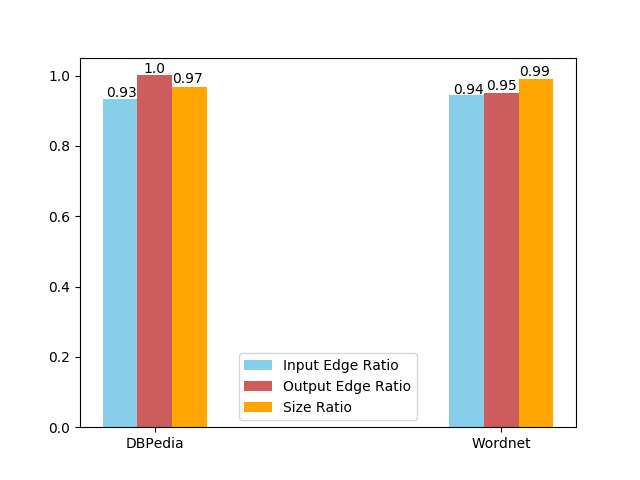
\includegraphics[width=0.8\linewidth]{figures/4_evaluation/ontology/ratiosSymmetricsDelete}
	\caption{Results for deleting symmetric properties, on the grammar level ($IER$, $OER$) and on the file size level ($SR$).}
	\label{fig:symmetricDeleteResults}
\end{figure}



The evaluation results are illustrated in Fig.~\ref{fig:symmetricAddResults2}. Of course, $IER>1$ is true and $IER$ is bigger than in Fig.~\ref{fig:symmetricAddResults}, since a higher amount of edges has been added. The fact that both $OER$ and $SR$ are lower than 1, supports our hypothesis that adding symmetric edges is more beneficial than removing them. So, we conclude that adding symmetric edges enables $Graph_{GRP}$ to find more digrams, and thus producing a smaller graph.

\begin{figure}
	\centering
	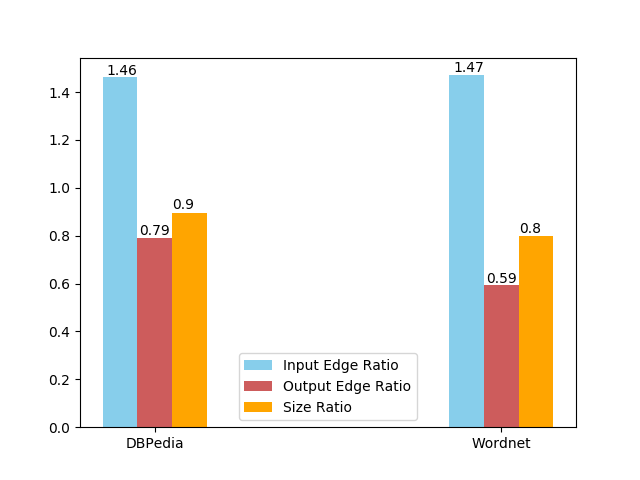
\includegraphics[width=0.8\linewidth]{figures/4_evaluation/ontology/ratiosSymmetricsAdd2}
	\caption{Results for adding symmetric properties, on the grammar level ($IER$, $OER$) and on the file size level ($SR$). In contrast to Fig.~\ref{fig:symmetricAddResults}, the input graph $in_1$ contains only one direction for each triple with a symmetric property.}
	\label{fig:symmetricAddResults2}
\end{figure}

\clearpage
\subsubsection{Inverse Properties}

Next, the usage of inverse properties is evaluated. First, the approach presented in Ch.~\ref{sec:approachInverse} (adding triples with inverse properties) is considered. Here, $DB_{inv}$ and $WN_{inv}$ have been used for DBPedia and Wordnet, respectively. The results are shown in Fig.~\ref{fig:inverseAddResults}. For DBPedia, the size of the input graph has been doubled ($IER=2.1$). But $OER=0.99$ is almost 1, thus the manipulation has not resulted in a better compression for DBPedia. $SR$ is even bigger than 1, so the end result is worse on the file size level.

For Wordnet, $IER$ is smaller than for DBPedia and more importantly, $OER$ is significantly smaller than 1. Hence, in this case, the manipulation has delivered a positive result. On the file size level, the result is also better ($SR=0.9$).

\begin{figure}
	\centering
	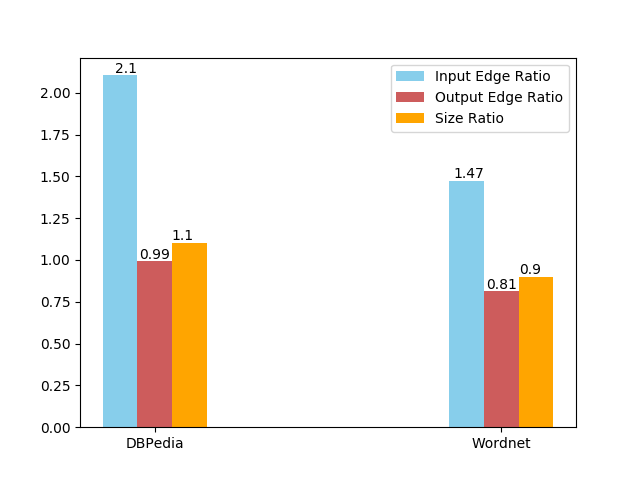
\includegraphics[width=0.8\linewidth]{figures/4_evaluation/ontology/ratiosInverseAdd}
	\caption{Results for adding inverse properties, on the grammar level ($IER$, $OER$) and on the file size level ($SR$).}
	\label{fig:inverseAddResults}
\end{figure}

In the case of DBPedia, a reason for the negative result can be that DBPedia has a relatively high number of different inverse properties. Therefore, adding all the edges with many different URIs to the relatively small graph in Fig.~\ref{fig:inverseAddResults} (1097 triples) does not have an effect that is positive enough to compensate the high amount of edges added to it. In order to further investigate that, a graph that is ten times bigger, is created. The results for it are shown in Fig.~\ref{fig:inverseAddResultsBigger} which are much better. While $IER$ is about 2 again, $OER=0.85$ is much smaller and also $SR=0.91$ is smaller. So, it can be stated that adding inverse properties has a positive effect on the graph compression potential, as mentioned in Ch.~\ref{sec:approachInverse}.


\begin{figure}
	\centering
	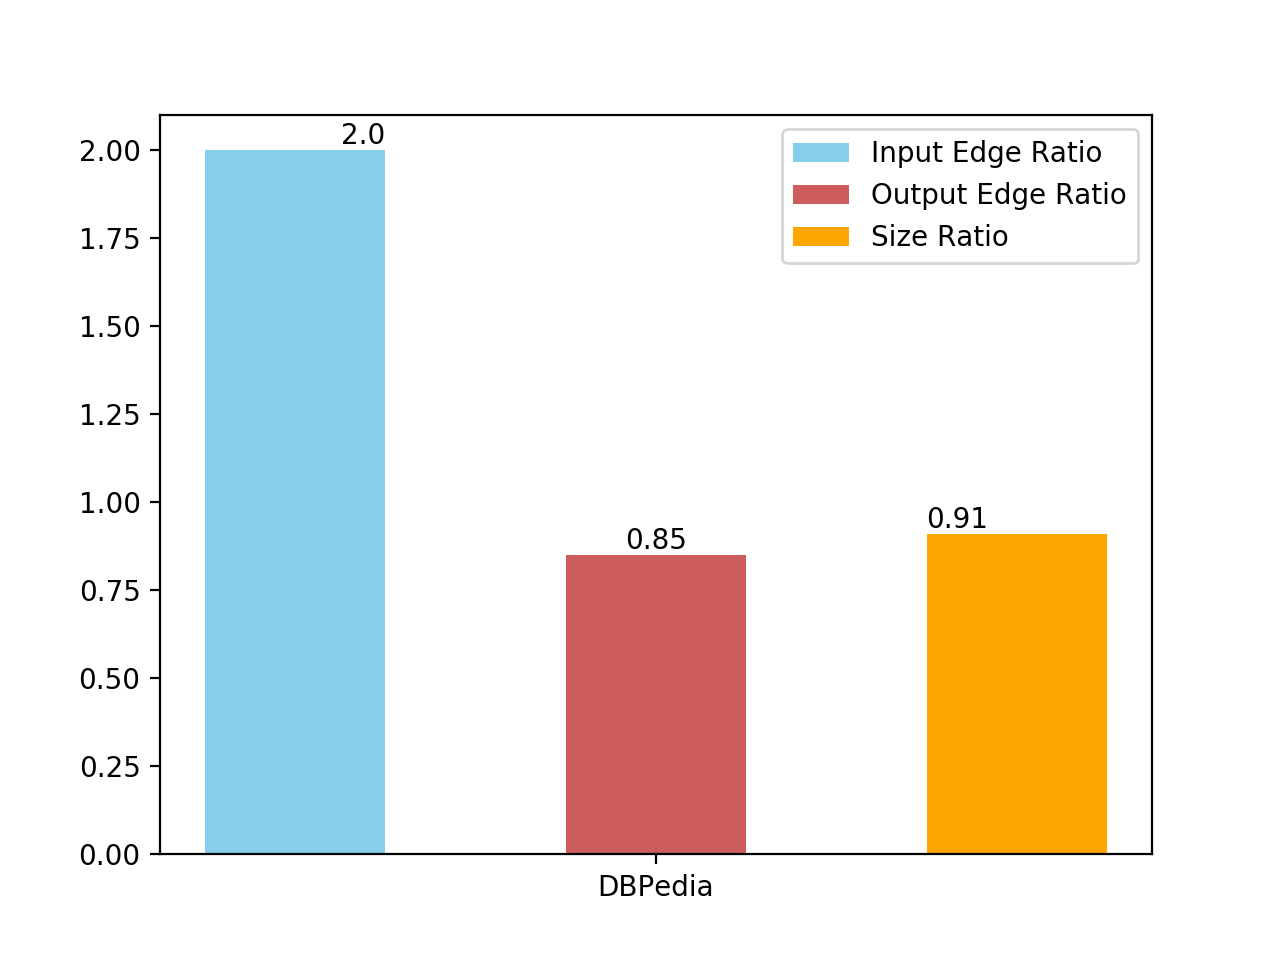
\includegraphics[width=0.8\linewidth]{figures/4_evaluation/ontology/ratiosInverseAddBigger}
	\caption{Results for adding inverse properties, on the grammar level ($IER$, $OER$) and on the file size level ($SR$). DBPedia graph is now 10 ten times bigger than in Fig.~\ref{fig:inverseAddResults}.}
	\label{fig:inverseAddResultsBigger}
\end{figure}

\begin{figure}
	\centering
	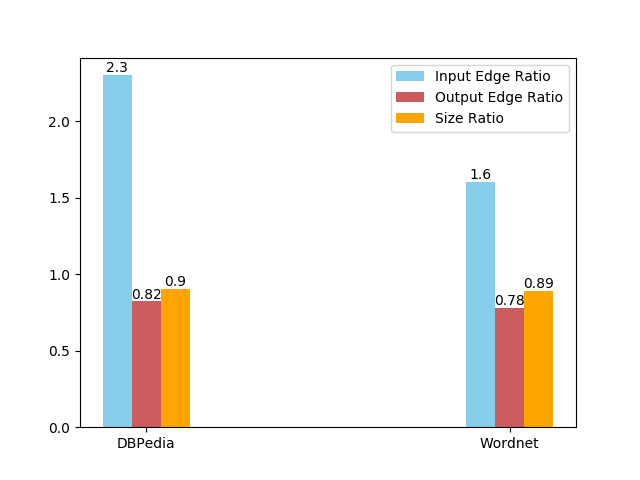
\includegraphics[width=0.8\linewidth]{figures/4_evaluation/ontology/ratiosInverseAdd2}
	\caption{Results for adding inverse properties, on the grammar level ($IER$, $OER$) and on the file size level ($SR$). In contrast to Fig.~\ref{fig:inverseAddResults} and~\ref{fig:inverseAddResultsBigger}, the input graph $in_1$ contains only one direction for each triple with an inverse property.}
	\label{fig:inverseAddResults2}
\end{figure}


The opposing approach (removing triples with inverse properties) is evaluated as well. Thus, the same technique, which was already used for symmetric properties, is used again. Hence, for DBPedia the graph $out_2$ of Fig.~\ref{fig:inverseAddResultsBigger} is used as $in_1$ and for Wordnet the graph $out_2$ of Fig.~\ref{fig:inverseAddResults} is used as $in_1$. The results are illustrated in Fig.~\ref{fig:inverseAddResults2}. There, it can be seen that the values for $IER$ are higher than before, as expected. Correspondingly, the $OER$-values are lower, which supports the hypothesis that removing inverse triples leads to an unfavorable graph structure for GRP.


\subsubsection{Transitive Properties}

The final evaluated ontology-based manipulation is adding or removing triples with transitive properties. The problem with the transitive case is that it is more restrictive than the others (symmetric or inverse). It is therefore more difficult to find data where this manipulation can be executed. In $DB_{tra}$, there are no \tps (defined in Ch.~\ref{sec:approachTransitive}). Thus, only $WN_{tra}$ will be used here, since it contains \tpsp

First, the approach suggested in Ch.~\ref{sec:approachTransitive}, to remove \textit{direct transitive paths}, is evaluated. Unfortunately, those edges do not exist in Wordnet. To circumvent that problem, an artificial graph has been created in the following way:  The original graph has been divided into two halves (via its list of triples). In the first half, all possible \dtps are added. Afterwards, the manipulated first half is merged with the untouched second half again. This gives us a graph in which both adding and removing \dtps is possible. So, both approaches can be evaluated.

The results for removing \dtps can be seen in Fig.~\ref{fig:ratiotransitivesDelete}. $IER$ is about 0.75, as several edges have been removed. $OER$ is about 0.5, which means that the removals have delivered a significant improvement on the grammar level. It could be argued that the improvement is only due to the reduced size of the graph. But this is not the case, since $OER<IER$ holds. Hence, due to the removed \textit{direct transitive paths}, $Graph_{GRP}$ could indeed find more digrams, as stated in Ch.~\ref{sec:approachTransitive}. On the file size level, the improved compression is also visible, because $SR\approx0.88$ is less than 1. Again, the improvement is not as good as on the grammar level.

\begin{figure}
	\centering
	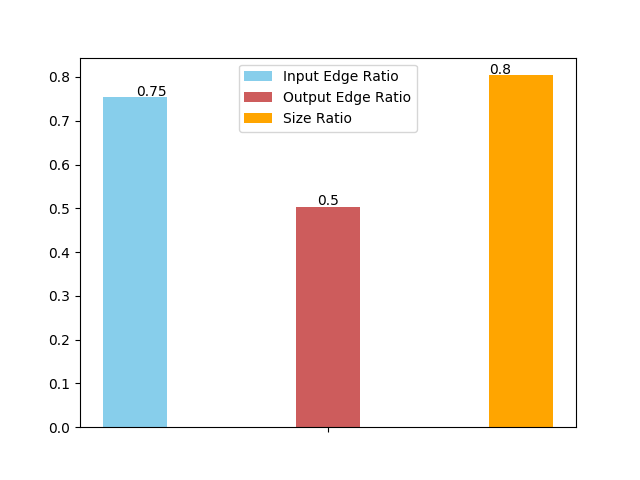
\includegraphics[width=0.8\linewidth]{figures/4_evaluation/ontology/ratioTransitivesDelete}
	\caption{$IER$, $OER$ and $SR$ for removing transitive edges in Wordnet.}
	\label{fig:ratiotransitivesDelete}
\end{figure}

Next, the opposing approach (adding \textit{direct transitive paths}) is evaluated. The results are illustrated in Fig.~\ref{fig:ratiotransitivesAdd}. Obviously, $ IER>1 $ holds, since many edges have been added. $OER\approx3.5$ is significantly high, which means that adding \dtps has resulted in a much larger result, on the grammar level. In contrast to Fig.~\ref{fig:ratiotransitivesDelete}, $IER<OER$ holds here, which supports the hypothesis that adding \dtps makes $Graph_{GRP}$ find less digrams (see Ch.~\ref{sec:approachTransitive}). On the file size level, $SR\approx1.8$ is higher than 1, but the result is not as bad as on the grammar level. 

Thus, it can be concluded that removing \dtps results in a better compression, and adding them delivers a worse compression. Although \dtps do not exist in the considered datasets, they still can exist in other datasets. The evaluation results have shown that removing \dtps leads to a insignificant improvement. 

\begin{figure}
	\centering
	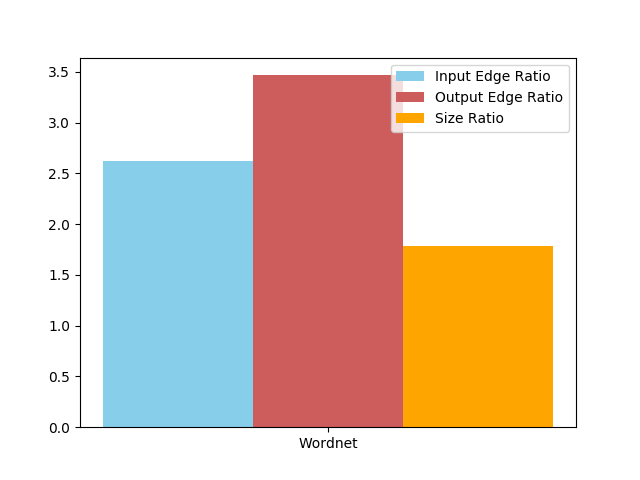
\includegraphics[width=0.8\linewidth]{figures/4_evaluation/ontology/ratioTransitivesAdd}
	\caption{$IER$, $OER$ and $SR$ for adding transitive edges in Wordnet.}
	\label{fig:ratiotransitivesAdd}
\end{figure}


\subsection{Dictionary Improvements}\label{sec:evaluationDictImprovements}

In this chapter, the approaches from Ch.~\ref{sec:implementationDictImprovements} which are intended to improve the dictionary compressor \DHDT{} (which is used by HDT and GRP), are evaluated. First, the Huffman compression of literals is evaluated and afterwards, the improvements regarding blank node IDs are discussed. 

\subsubsection{Dataset Overview}

Tab.~\ref{tab:HuffImproveDatasets} shows the datasets which were used for evaluating the Huffman improvements. $ELR$ and $SPS$ are not shown here, since they are not relevant for the dictionary compression. Moreover, the datasets used in Ch.~\ref{sec:evaluationLiterals} (with the names DF0-DF9) are the same as in Tab.~\ref{tab:comparisonDatasets} and are therefore not shown in Tab.~\ref{tab:HuffImproveDatasets}.

Tab.~\ref{tab:BlankImproveDatasets} shows the files used for the blank node improvements. Here, also the number of triples with blank nodes is presented (includes triples with at least one blank node).

\begin{center}
	\begin{tabular}{|c|c|c|c|}
		\hline 
		Short Name & Long Name & \#Triples & \#Resources \\ 
		\hline
		AB\_EN & long-abstracts\_en\_small & 10000 & 10000 \\
		\hline
		AB\_BG & long-abstracts-en-uris\_bg\_small & 10000 & 10000  \\
		\hline
		AB\_FR & long-abstracts-en-uris\_fr\_small & 10000 & 10000 \\
		\hline
		AB\_RU & long-abstracts-en-uris\_ru\_small & 10000 & 10000 \\
		\hline
	\end{tabular} 
	\captionof{table}{RDF files for the Huffman evaluations. URLs to the datasets are in Ch.~\ref{sec:implementationDatasets}.}	
	\label{tab:HuffImproveDatasets}
\end{center}

\pagebreak
\begin{center}
	\begin{tabular}{|c|c|c|c|c|}
		\hline 
		Short Name & Long Name & \#Triples & \#Resources & \#Triples with blank nodes \\ 
		\hline
		GC1 & DEE\_geometry & 213 & 12 & 211 \\
		\hline
		GC2 & PL1\_geometry & 357 & 12 & 355 \\
		\hline
		GC3 & TR2\_geometry & 280 & 14 & 278 \\
		\hline
	\end{tabular} 
	\captionof{table}{RDF files for the blank node evaluations. URLs to the datasets are in Ch.~\ref{sec:implementationDatasets}.}	
	\label{tab:BlankImproveDatasets}
\end{center}



\subsubsection{Literals}\label{sec:evaluationLiterals}

As already mentioned, a self-generated Huffman code was used to compress the literals of an RDF graph, as it is likely to get a better compression than with the prefix-based compression of HDT.

Thus, the results of the evaluation are presented. First, the Semantic Web Dog Food data set is used. This is well suited for an evaluation, since both literals and URIS are included here. Fig.~\ref{fig:dogfoodcomprratiosSub} shows \CRDict{HDT} for a subset of the data (DF0 - DF9). 

It can be seen that the usage of the Huffman code only brings a small improvement in some cases. In some cases Normal \DHDT{} even compresses better than \DHDT{} with Huffman.

This is because the data does not have a very high proportion of literals. Also, literals are rather short here. This can be seen in Fig.~\ref{fig:dogfoodliteralanalysis} showing the relative literal amount ($\frac{\#literals}{\#triples}$) and the average length of a literal. The proportion of literals in the triples is never higher than 17.5\% and the highest average literal length is about 12. Hence, these are single words rather than whole texts. Only in cases where both the proportion and the literal length are relatively high, an improvement can be seen (e.g. DF9).


\begin{figure}[h]
	\centering
	\subfloat[$CR(out_{dict})$ for Normal HDT and HDT + Huffman]{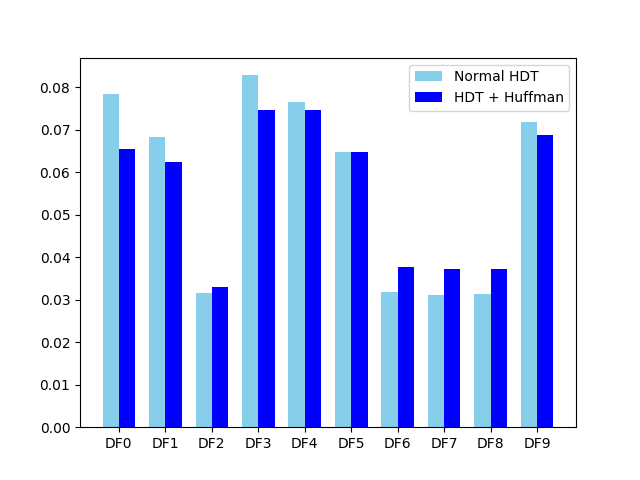
\includegraphics[width=\subfigWidth\textwidth]{figures/4_evaluation/dogFoodComprRatios}\label{fig:dogfoodcomprratiosSub}}
	\hfill
	\subfloat[Relative amounts of literals and average literal length.]{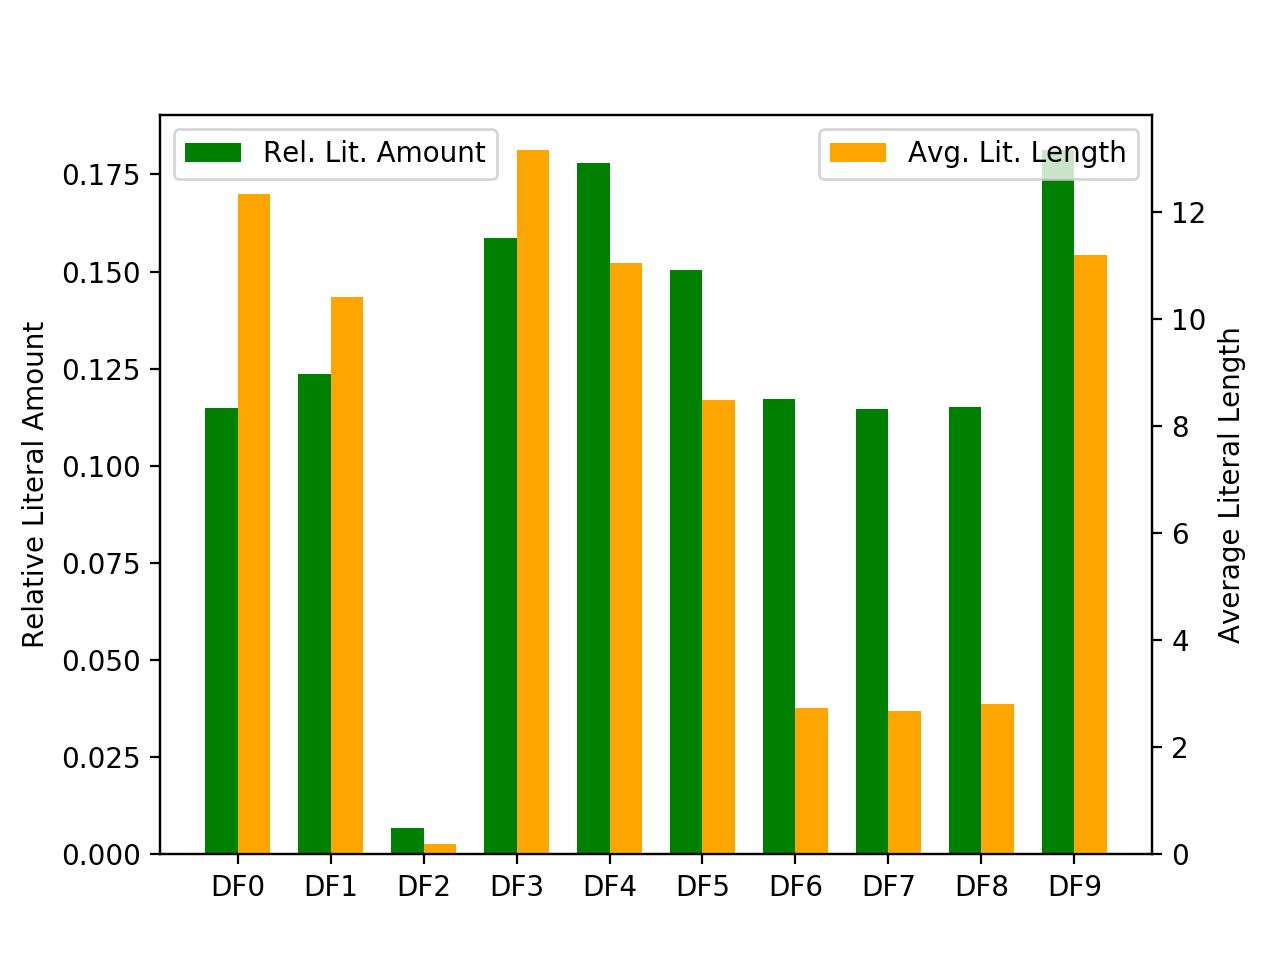
\includegraphics[width=\subfigWidth\textwidth]{figures/4_evaluation/dogFoodLiteralAnalysis}\label{fig:dogfoodliteralanalysis}}
	\caption{Compression ratios~(\ref{fig:dogfoodcomprratiosSub}) and features of the same files~(\ref{fig:dogfoodliteralanalysis}) from Semantic Web Dog Food.}
	\label{fig:dogfood}
\end{figure}


Next, the DBPedia data set is considered, because it has a different structure of data. Here, graphs are considered which contain the abstracts of Wikipedia, because these are longer texts. In addition, there are abstracts in different languages, so it can be seen whether some languages are better suited for Huffman than others.

Fig.~\ref{fig:dbAbstractscomprratiosSub} shows \CRDict{HDT} for the abstract files. The abbreviations stand for the languages the abstracts are written in. It can be seen that Huffman significantly improves \CRDict{HDT} here. The reason for this can be seen in Fig.~\ref{fig:dbAbstractsliteralanalysis}, where the average literal length is illustrated. The relative literal amount is not shown this time, since it is 100\% for all files. The average literal length varies between languages, but is generally much higher than in Semantic Web Dog Food. Therefore, the improvement is much greater here.

Another phenomenon can also be seen here: Although the English file contains the longest literals by far, the improvement by Huffman here is not as big as, for example, in the Bulgarian file. In the English case, the Huffman code is less effective, because there are fewer different characters than in the other languages. Huffman is generally more efficient on large alphabets, according to~\cite{huffman}.

\begin{figure}[h]
	\centering
	\subfloat[$CR(out_{dict})$ for Normal HDT and HDT + Huffman.]{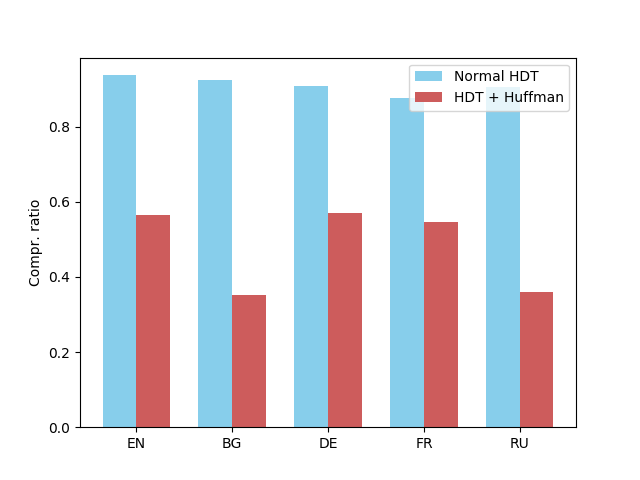
\includegraphics[width=\subfigWidth\textwidth]{figures/4_evaluation/dbAbstractsComprRatios}\label{fig:dbAbstractscomprratiosSub}}
	\hfill
	\subfloat[Average literal length.]{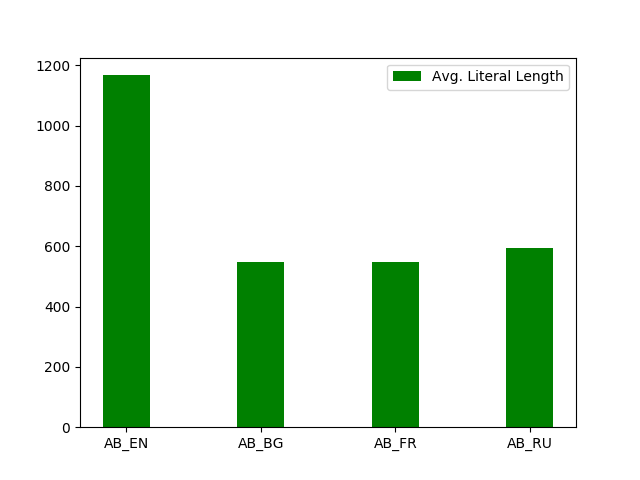
\includegraphics[width=\subfigWidth\textwidth]{figures/4_evaluation/dbAbstractsLiteralAnalysis}\label{fig:dbAbstractsliteralanalysis}}
	\caption{Compression ratios~(\ref{fig:dbAbstractscomprratiosSub}) and features of the same files~(\ref{fig:dbAbstractsliteralanalysis}) from DBPedia.}
	\label{fig:dbAbstracts}
\end{figure}

As mentioned above, saving the Huffman code means almost no additional storage effort. The average fraction of the Huffman code is about 0.1\% and was therefore not displayed in the visualizations.

Since the calculation of the Huffman code increases the runtime of the whole compression, it is now considered how big this effect is. Fig.~\ref{fig:dbAbstractsRuntimes} shows $CT$ for the compression of the DBPedia abstract data. Here, $CT$ has been increased very much. This is because \DHDT{} can normally compress very little with this data, due to the numerous long literals and is therefore finished quite quickly. With Huffman the data can be compressed much better and it takes quite a long time. Here, especially the creation of the Huffman tree is expensive.

Fig.~\ref{fig:dogFoodRuntimes} shows $CT$ for the Semantic Web Dog Food data, where the run times are only slightly longer, because Huffman hardly improves the compression.

Generally, it can be said that the use of a standard Huffman code could be worthwhile because of the otherwise high runtime. At this point, however, the evaluation with such a standard code was omitted, since such existing codes do not contain all the special characters that occur in RDF data.


\begin{figure}[h]
	\centering
	\subfloat[$CT$ for DBPedia abstracts.]{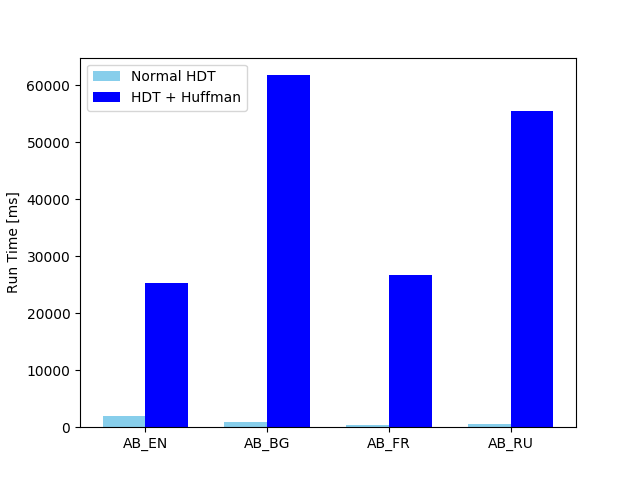
\includegraphics[width=\subfigWidth\textwidth]{figures/4_evaluation/dbAbstractsRuntimes}\label{fig:dbAbstractsRuntimes}}
	\hfill
	\subfloat[$CT$ for Semantic Web Dog Food files.]{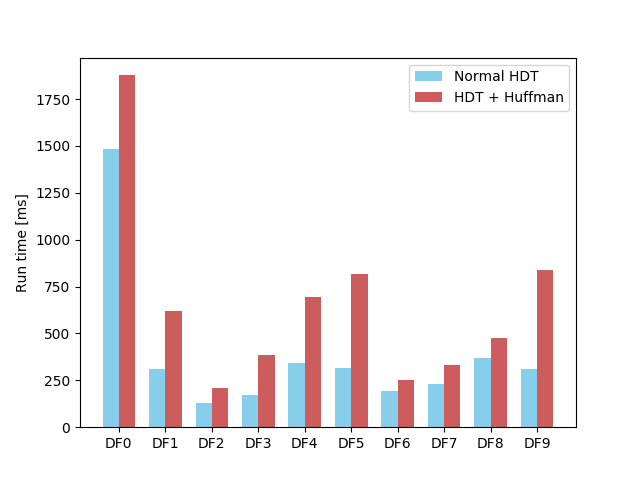
\includegraphics[width=\subfigWidth\textwidth]{figures/4_evaluation/dogFoodRuntimes}\label{fig:dogFoodRuntimes}}
	\caption{Run times ($CT$) for Normal HDT and HDT + Huffman.}
	\label{fig:huffmanRuntimes}
\end{figure}

\subsubsection{Blank Nodes}\label{sec:evaluationBlankNodes}

This chapter evaluates the two approaches mentioned in Ch.~\ref{sec:approachBlankNodes} to store blank node IDs more efficiently. For that, the Nuts-RDF dataset is used as it contains much more blank nodes than many other datasets. It is therefore prone to show the inefficiency of the prefix-based compression of $Dict_{HDT}$ with respect to blank nodes. Fig.~\ref{fig:blanknodes} shows the results for three different files from Nuts-RDF. It can be seen that Normal \DHDT{} even produces the result $CR_{Dict_{HDT}}>1$. This is due to the fact that GC1-GC3 are in the turtle format which already reduces redundancy, since it does not store all triples extensively, like N-Triples does. Also, it does not use blank node IDs that are as long as those used by $Dict_{HDT}$. Using short IDs already brings a significant improvement as it delivers a compression ratio between 0.76 and 0.89. So, the compression is now really reducing the size of the files. Omitting the blank node IDs results in further slight improvement which is small, because storing the short IDs as numbers from 1 to $n$ costs almost no memory size. Hence, it could be sufficient to use shorter IDs, because omitting IDs would imply more programming effort, as explained in Ch.~\ref{sec:implementationBlankNodes}.


\begin{figure}
	\centering
	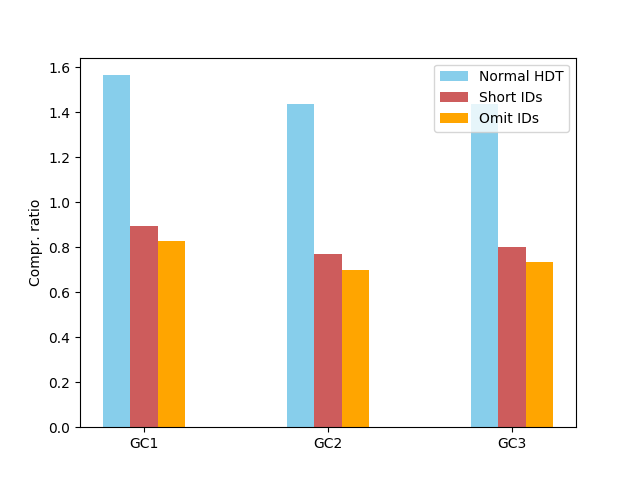
\includegraphics[width=0.8\linewidth]{figures/4_evaluation/blankNodes}
	\caption{Results for Blank Node ID improvements for Geo Coordinates (GC) files. \textbf{Normal HDT} uses long IDs. \textbf{Short IDs} uses integer IDs. \textbf{Omit IDs} does not store the IDs at all.}
	\label{fig:blanknodes}
\end{figure}

\FloatBarrier
\subsection{Final Results}\label{sec:evaluationFinal}

\begin{figure}
	\centering
	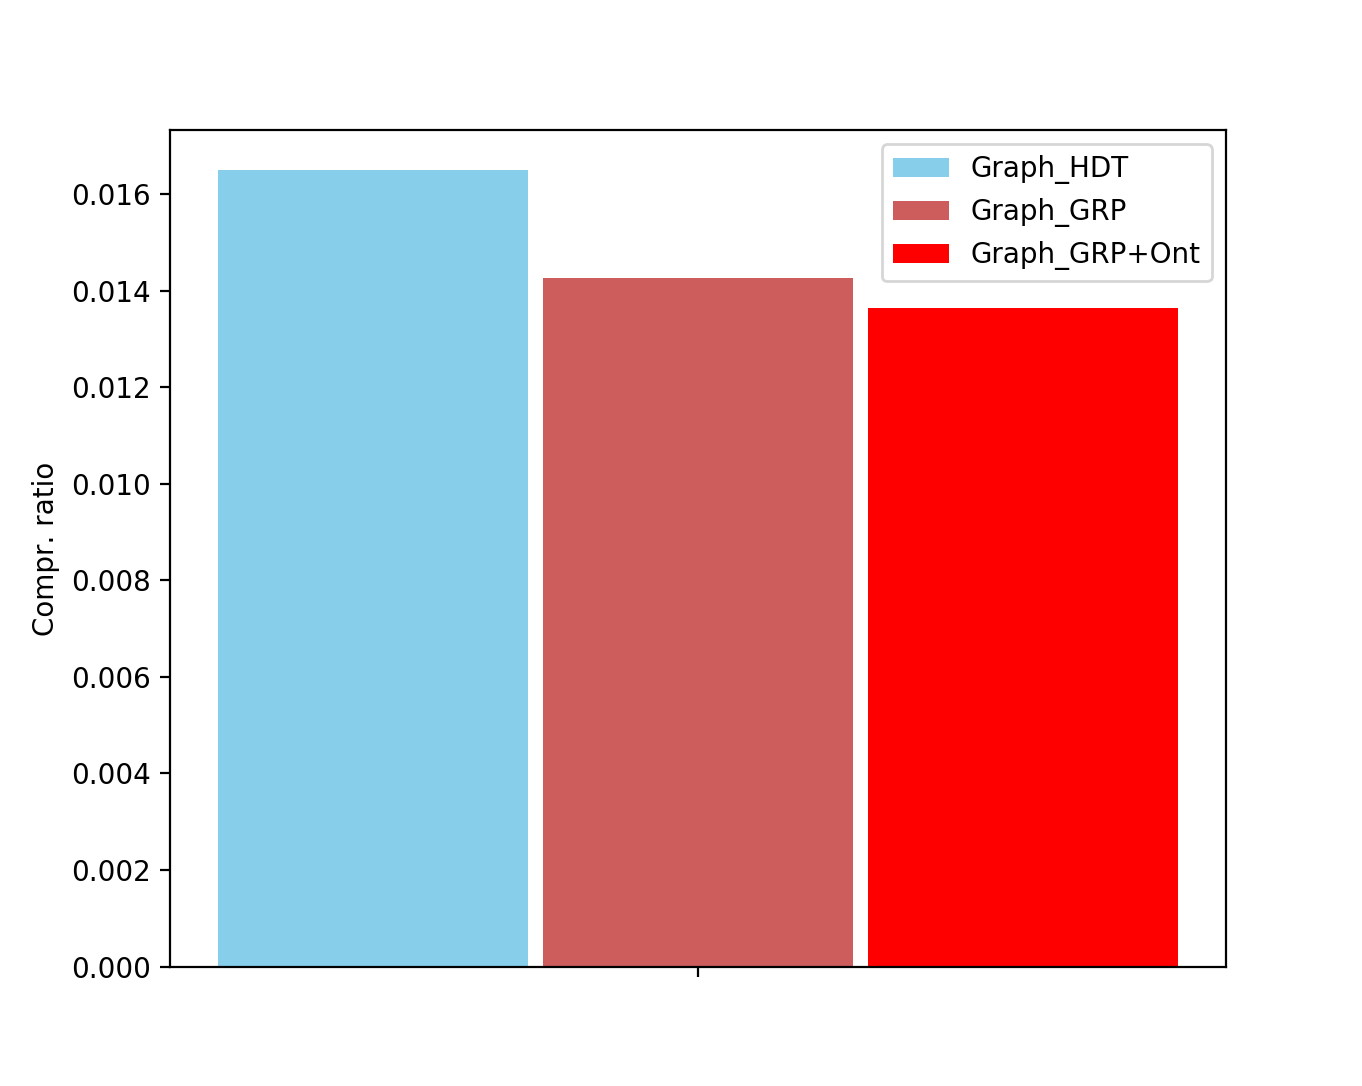
\includegraphics[width=0.6\linewidth]{figures/4_evaluation/final/graphcompr}
	\caption{Graph compression ratios ($CR_{Graph_C}$) for $Graph_{HDT}$, $Graph_{GRP}$ and $Graph_{GRP+Ont}$.}
	\label{fig:graphcompr}
\end{figure}


In the previous chapters, the compression improvements (graph and dictionary) were evaluated individually. This final evaluation chapter compares all improvements together. This makes it possible to see which improvement accounts for which portion of the overall improvement. 

In order to realize this, an RDF graph is generated from several graphs. The graph $DB_{inv}$ from Tab.~\ref{tab:ontologyKnowledgeDatasets} serves as a basis, as it contains inverse and symmetric properties. However, there are not many long literals in it. Therefore, the DBPedia abstract text is added for each person in the graph (from the abstract data set from Ch.~\ref{sec:evaluationLiterals}). Next, blank nodes are added to the graph. Thus, the coordinates (polygons) for each country of the graph are added. The data set from Ch.~\ref{sec:evaluationBlankNodes} is used for that. Finally, this results in a graph on which all improvements have an effect. In Tab.~\ref{tab:finalDataset}, the features of that graph can be seen.

\begin{center}
	\begin{tabular}{|c|c|c|c|c|}
		\hline 
		 \#Triples & \#Resources & \#Literals & \#Triples with blank nodes \\ 
		\hline
		101193 &59565 & 6058 & 230 \\
		\hline 
	\end{tabular} 
	\captionof{table}{RDF file for the final evaluations.}	
	\label{tab:finalDataset}
\end{center}

\FloatBarrier
Fig.~\ref{fig:graphcompr} shows the graph compression improvements. For the ontology-based improvement of $Graph_{GRP}$ we write $Graph_{GRP+Ont}$.  It can be seen that $Graph_{GRP}$ already compresses better than $Graph_{HDT}$. $Graph_{GRP+Ont}$ brings only a small improvement. This due to the encoding problem discussed in Ch.~\ref{sec:evaluationOntKnowledge}.

Fig.~\ref{fig:dictcompr} shows the results regarding the dictionary compression. By $Dict_{HDT++}$, the improved HDT dictionary compression (literals and blank node IDs) is denoted. Here, the improvement is significant although the used RDF graph does not contain as much literals as the abstract graphs used in Ch.~\ref{sec:evaluationLiterals}. 

Finally, Fig.~\ref{fig:completecompr} shows both the graph and dictionary compressions in combination. HDT++ denotes the improved HDT (HDT++$=\{  Dict_{HDT++}, Graph_{HDT} \} $). GRP++ denotes the ontology-based graph compression improvement combined with the improved dictionary compression (GRP++ $=\{ Dict_{HDT++}, Graph_{GRP+Ont} \}$). The horizontal lines drawn through the bars denote the respective values of $CR_{Dict_C}$. That shows how big the portion of the dictionary is in the compressed data. 

Apart from that, the difference between HDT++ and GRP++ is very small. This due to the fact that the graph ($out_{graph}$) is so much smaller than $out_{dict}$.

GZip is used a baseline. Since it is a general compressor, it does not have a horizontal line. It is noticeable that GZip achieved a slightly better compression ratio than HDT++ and GRP++. However, as already mentioned in Ch.~\ref{ch:introduction}, the data compressed by GZip is not query-able which makes it less usable.

In general, it can be concluded that the improvement makes a significant difference. The resulted compression ratio is almost as low as GZip's ratio. Considering the fact that data compressed by GRP++ or HDT++ is still query-able, it is reasonable to use one of them instead of a general compressor. With further improvements (will be discussed in Ch.~\ref{sec:futurework}) it could be that HDT++ or GRP++ outperform general compressors in many more cases.

Moreover, it becomes clear that compressing the dictionary has a much bigger impact on $CR_C$ than compressing the graph. So, for future work it would be reasonable to focus on dictionary compression. However, one work around could be to compress multiple RDF files, which all have a similar dictionary, together. This way, the influences of the graphs can become bigger.



\begin{figure}
	\centering
	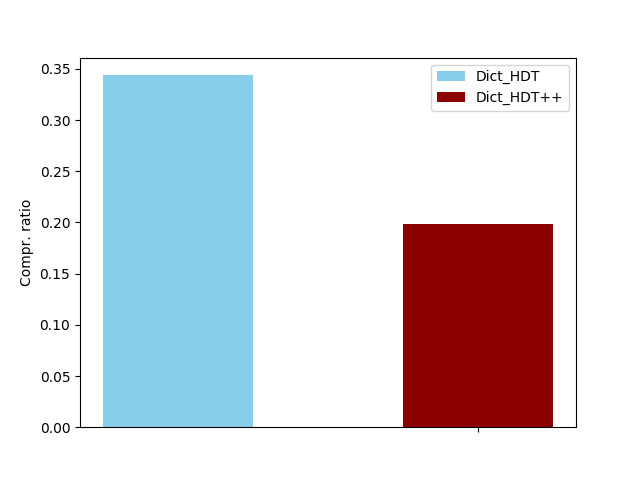
\includegraphics[width=0.8\linewidth]{figures/4_evaluation/final/dictcompr}
	\caption{Dictionary compression ratios ($CR_{Dict_C}$) for $Dict_{HDT}$ and $Dict_{HDT++}$.}
	\label{fig:dictcompr}
\end{figure}





\begin{figure}
	\centering
	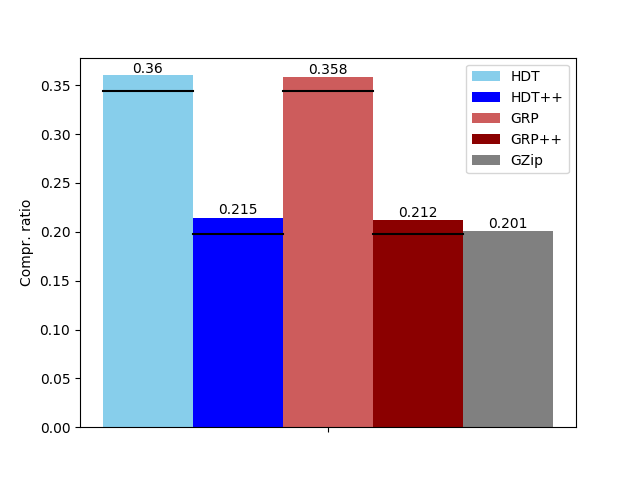
\includegraphics[width=0.8\linewidth]{figures/4_evaluation/final/completecompr}
	\caption{Complete compression ratios ($CR_C$) for all compressors. Horizontal lines mark the values of $CR_{Dict_C}$. GZip is used as a baseline.}
	\label{fig:completecompr}
\end{figure}
















